\documentclass[11pt]{amsart}
\usepackage{geometry}           % See geometry.pdf to learn the layout options. There are lots.
\geometry{letterpaper}          % ... or a4paper or a5paper or ... 
%\geometry{landscape}           % Activate for for rotated page geometry
%\usepackage[parfill]{parskip} 	% Activate to begin paragraphs with an 
								% empty line rather than an indent
\usepackage{graphicx}
\usepackage{amssymb}
\usepackage{epstopdf}
\usepackage{tikz-qtree}
\usepackage{graphicx}
\usepackage[table,xcdraw]{xcolor}
\usepackage{tikz}

\usepackage{algpseudocode}
\usepackage{algorithm}

\usepackage{hyperref}% http://ctan.org/pkg/hyperref                                                                                                                                                         
\usepackage{cleveref}% http://ctan.org/pkg/cleveref                                                                                                                                                     \biboptions{}    

\usetikzlibrary{arrows,automata}
\usepackage{enumitem}

%---------------------- For System Architecture -------------------------------------------%
\usetikzlibrary{positioning,calc,fit,mindmap,trees}

\definecolor{mybluei}{RGB}{124,156,205}
\definecolor{myblueii}{RGB}{73,121,193}
\definecolor{mygreen}{RGB}{202,217,126}
\definecolor{mypink}{RGB}{233,198,235}

% this length is used to control the width of the light blue frame
% for the upper part of the diagram
\newlength\myframesep
\setlength\myframesep{8pt}

\pgfdeclarelayer{background}
\pgfsetlayers{background,main}

\pgfkeys{
  /tikz/node distance/.append code={
    \pgfkeyssetvalue{/tikz/node distance value}{#1}
  }
}

\newcommand\widernode[5][blueb]{
  \node[
    #1,
    inner sep=0pt,
    shift=($(#2.south)-(#2.north)$),
    yshift=-\pgfkeysvalueof{/tikz/node distance value},
    fit={(#2) (#3)},
    label=center:{\sffamily\bfseries\color{white}#4}] (#5) {};
}
%---------------------- End of System Architecture ----------------------------------------%

\DeclareGraphicsRule{.tif}{png}{.png}{`convert #1 `dirname #1`/`basename #1 .tif`.png}

\title{Proposition of Volunteer Cloud Computing}
\author{Dany Wilson}
%\date{}                                         % Activate to display a given date or no date

\begin{document}
\maketitle
        \section{Introduction}
	In this current era we can see a shift in how software and hardware are conceived, the end-
	goals are not the same as they used to be 2 decades ago. This can be attributed to the 
	following, the fact that the Internet speed got a lot faster, by a factor of 1000 (based on
	a 56kbps connection in 1995, compared to a 50mbps connection today), but also because the 
	hardware performance augmented at a similar pace. Initially in the pre-Internet era, 
	software was written to be executed locally without any network interactions. Then in the 
	genesis of the Internet, the objectives of software slowly shifted to access external 
	resources, thus the apparition of the e-mail and the web-browser. Slowly as the connection
	bandwidths increased, there was an increased number of possible usage such as online games, 
	content streaming, social-media, etc. Nowadays we can access fully virtualized computing
	environments within our web-browsers, and this takes us the very genesis of the Cloud 
	Computing era. 

	\subsection{The Genesis of Cloud Computing}
	The embodiment of Cloud Computing, namely the Internet of Things, can actually be traced 
	back to the vision of J.C.R. Licklider of the \emph{"Intergalactic Computer Network"} 
	\cite{licklider}:
	\begin{quote}
		At this extreme, the problem is essentially the one discussed by science fiction 
		writers: \emph{"how do you get communications started among totally uncorrelated 
		sapient beings?"}
	\end{quote}
	This quote shows us the state of electronic tele-communication in the sixties, which is 
	described as being fabric of fiction. There was military but also academic interest of 
	providing an infrastructure that supports long-distance information processing. One of the most 
	interesting idea of this memorandum is best conveyed in this following quote:
	\begin{quote}
		When the computer operated the programs for me, I suppose
		that the activity took place in the computer at SDC, which
		is where we have been assuming I was. However, I would just
		as soon leave that on the level of inference. With a
		sophisticated network-control system, I would not decide
		whether to send the data and have them worked on by
		programs somewhere else, or bring in programs and have them
		work on my data. I have no great objection to making that
		decision, for a while at any rate, but, in principle, it
		seems better for the computer, or the network, somehow, to
		do that.
	\end{quote}
	This very quote reflects the concept of offloading, not only of information or data, but 
	of computation as a service. In other words that in some case it would be better, given the 
	proper networking infrastructure, to offload the computation and send the data to be 
	processed remotely.
	
	Around the same time the concept of virtualization was being explored in the context of 
	mainframe computers, in order to logically divide the resources between applications 
	allowing them to run simultaneously. Throughout the years, the concept of virtualization 
	broaden and now it is possible to run a complete Operating System on the application level.
	There is a direct correlation with the coming of the virtualization of hardware and the 
	birth of the Cloud. 
	
	Cloud Computing is heavily influenced by the maturity of the Service-Oriented Architecture, 
	and as we said earlier the evolution of the "Internet" with respect to the Web 2.0. That 
	evolution of the Web from 1.0 to 2.0 is marked by the following characteristics, as cited in 
	\cite{web20}: \emph{[...] services, not packaged software, with cost-effective scalability; 
	[...] data-centric w.r.t. Big Data; [...] users as co-developers; [...] harnessing collective 
	intelligence; [...] leveraging long-tail effect through customer self-service.} We can observe 
	a trend, the concept (web) services (rather then serving only static content) but also how 
	the user becomes the central point of the network as a platform. This entails that components 
	of the Web are becoming interactive services that can be contracted to responds to the users 
	needs, via real-time aggregation of information using Big Data.

	Thus the Cloud is the natural evolution of utilizing the network as a platform, through a 
	Service-Oriented Architecture with respect to the natural evolution and maturity of the 
	Web entailing the definition and wide-spread usage of mature Web-Services homogeneous 
	interface (API). \emph{Ipso Facto}, the adoption of pay-per-use business model for the 
	offerings of Cloud Infrastructure.
	
	% Need to talk about its similarities between the SOA, distributed, grid computing...
	%
	\subsection{The Cloud}
	There have been numerous attempts to try to give a concise or approximate picture of the 
	Cloud Computing paradigm, with respect to its implementation and its different business 
	models. One can review the following, \cite{soa_cloud}, \cite{vaquero}, \cite{ontology},\cite{panzieri}; 
	to name a few. We feel that \cite{nist}, \cite{soa_cloud} and \cite{ontology}, provides a 
	clear enough picture to represent the current Cloud ecosystem and we will use them to do so.
		
	Cloud Computing infrastructure offers many advantages compared to the traditional on-premise 
	infrastructure and it is why numerous companies consider outsourcing their IT infrastructure to 
	an off-premise solution. Among the most important characteristics that this type of 
	infrastructure offers, the NIST enumerates the following five \cite{nist}:
	\begin{enumerate}
		\item{\textbf{On-demand Self-service}} \emph{Consumers are not required to interact with 
		any representative of the provider to provision computing capabilities, rather it is 
		automated through the provider's infrastructure.}\\
		\item{\textbf{Broad Network Access}} \emph{Services are available over standard network 
		infrastructure and through standard	mechanisms, enabling different client platforms like 
		cell-phones, laptop, tablets, etc.}\\
		\item{\textbf{Resource Pooling}} \emph{Providers offers a pool of Resources to different 
		clients via a multi-tenant model, consisting of physical and virtual resources that can be 
		assigned and re-assigned dynamically to cater to the clients demands. Clients are only 
		aware, or able to choose the location of these resources with respect to pre-defined 
		geographical regions. }\\
		\item{\textbf{Rapid Elasticity}} \emph{Resources and services can be provisioned to scale 
		to meet the fluctuations of the client's needs at any time, at any magnitude. The provider
		offers a seemingly unlimited number of services and resources to the client.}\\
		\item{\textbf{Measured Service}} \emph{Resource usage can be monitored, controlled 
		(optimized) and reported in a manner that proves transparent to both provider and consumer.}
	\end{enumerate}
	
	In this modern day and age, among the major service providers of \emph{The Cloud} we can 
	find the likes of Google, Microsoft and Amazon, to name a few. They provide their services 
	as a 5 different service models:\\
	
	\begin{center}
		% Cloud Services graphic (may need to represent it better...)
		\begin{figure}[h]
			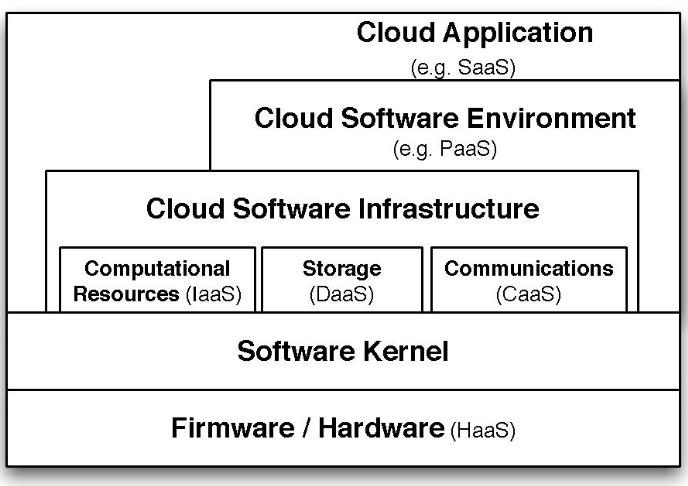
\includegraphics[width=125mm]{c_ontology.png}
			\caption{Ontological Representation of Cloud\label{c_ontology}}
		\end{figure}
	\end{center}
	
	Based on \cite{ontology}, we can appreciate the categorization that emerged from their study of 
	the major Cloud Service providers. We will briefly explain 3 of these categories in order to 
	have a clearer picture of where this proposition resides in the grand scheme of the Cloud. In 
	order to do so we will explore the question with respect of the Separation of Responsibilities, 
	via a very concise graphical depiction \cite{Blewis}:
	
	\begin{center}
		\begin{figure}[h]
			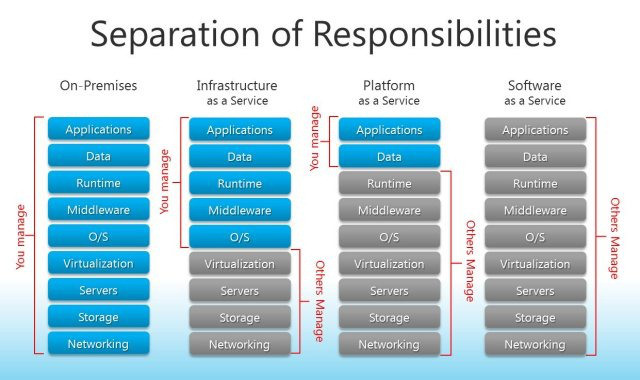
\includegraphics[width=125mm]{cloud_sep_of_resp.jpg}
			\caption{Cloud Services w.r.t. Responsibilities\label{cloud_sep_of_resp}}
		\end{figure}
	\end{center}
	
	\subsubsection{Infrastructure-as-a-Service (IaaS)}
	This service model provides, to its consumers, a virtualized environment that represents the 
	full stack, from the hardware-level to the software-level, while taking care of the hardware 
	management aspect. With this model, consumers can deploy any Operating System they wish, and as a
	matter of fact create the software environment that they deem most appropriate for their use. 
	Since the hardware management responsibility is left out to the service provider, the client can 
	easily augment or reduce the computing power at will to cope with the fluctuation of their 
	demands. Amazon's Elastic Cloud Compute (EC2), or Windows Azure are part of the available IaaS 
	solutions currently available.
	
	\subsubsection{Platform-as-a-Service (PaaS)}
	This service model, if we refer to Figure \ref{cloud_sep_of_resp}, to its clients the ability of 
	having to manage only the Application and Data aspect of the full-stack, everything else is \
	managed and taken care of by its provider. Using such a service the client can focus on simply 
	developing their application using the libraries, services and tools supported by the provider, 
	and then deploy it onto the Cloud. Google's App Engine is perhaps one of the most popular example 
	of this model.
	
	\subsubsection{Software-as-a-Service (SaaS)}
	This service model, the consumer is provided with the capability to use applications (or 
	software) running on the provider's cloud infrastructure, with little to no management 
	capability, as depicted in Figure \ref{cloud_sep_of_resp}. From a user's perspective application 
	are served as an atomic service, in the likes of Oracle ON DEMAND which offers on demand a 
	customer relationship management application.
	
	Finally we need to discuss the different \emph{Deployment Models} that are offered in the Cloud 
	eco-system. Relying again on the NIST \cite{nist} document, let's briefly present the 4 models:
	
	\begin{enumerate}
		\item{\textbf{Private Cloud}} \emph{This cloud infrastructure is meant to be used by a single 
		organization, which can act also as a single provider or a providing partner with a 3rd party 
		or solely as a consumer. Exclusivity is the key here.}\\
		\item{\textbf{Community Cloud}} \emph{Very similar to the private cloud model, but in this 
		case exclusivity of usage is shared among a community sharing common interests.}\\
		\item{\textbf{Public Cloud}} \emph{This deployment model is aimed for open use by the general 
		public, and the embodiment of this model's infrastructure is known as a Cloud Provider, such 
		as Amazon, Google, Windows, etc.}\\
		\item{\textbf{Hybrid Cloud}} \emph{This is the result of the combination of two or more 
		distinct cloud infrastructure (which remain distinct to one another), but are combined using 
		standardized or proprietary technologies to enable data and application portability.}
	\end{enumerate}
	
	In the following subsection we will present a fifth deployment model, namely Volunteer Cloud 
	Computing. But in order to provide the proper context for its emergence, lets take a brief look
	at Grid Computing and Volunteer Computing.
	
	\subsection{Grid Computing}
	A very extensive literature exist on this fairly recent paradigm (cite proper sources), and we 
	can define it as being a form of Distributed Computing, where each node is ask to perform a 
	different task, and the aggregation of those nodes workload constitutes the workload that needs 
	to be perform in order to achieve the goal of (computationally) realizing its mandate. A
	
	\subsection{Volunteer Computing}
	The @Home paradigm or philosophy beautifully proves how this is realized, and let's look at a 
	simple example the SETI@Home project.
	
	%mention panzieri for its representation of different cloud topologies.
	
	\subsection{Volunteer Cloud Computing}
	The concept of Volunteer Cloud Computing is a fairly new one, since as we can see there is no 
	mention of it whatsoever in \cite{nist}\cite{taxonomy}. It revolves around user-provided 
	resources as the building components of the cloud infrastructure, and typically takes place in 
	a decentralized manner for which no single provider is designated, rather the collection of the
	participants form at the same time the provider and the consumers. One of the driving factors of 
	this topological ideology is to harvest and make efficient use of distributed idling 
	resources to provide a cloud infrastructure, with no real added cost. 
	
	In the following section we will review the literature to find out more about the position of 
	Volunteer Cloud Computing with respect to the current deployment models in place, and if any 
	implementation exists.
	
	\section{Related Work}
	
	\subsection{Cloud@Home}
	The first real apparition of the term Volunteer Cloud Computing can be attributed to 
	\cite{cathome}, in 2009 when they proposed the Cloud@Home paradigm. It can be described as a 
	continuation of the @Home distributed computing effort and the merging of volunteer computing and 
	Cloud computing. They propose an infrastructure in which it is possible for heterogeneous 
	computing resources to be connected and to co-operatively provide a Cloud infrastructure, at a 
	cost or for free. Thus this is a leap into monetizing the idle time of the consumer-grade 
	computing resources, to provide a seamless Cloud experience to consumers. Although they provide a 
	very detail analysis of the majority of the factors present in a Cloud architecture, little to no 
	information was released after the publication of a series of more specific papers on the 
	subject,.
	%\cite{cathome2}.
	Last paper that was published, \cite{cathome11}, was indicating that they were actively working on 
	an implementation of their proposed framework, but that was back in 2012. Thus, we will elaborate 
	on what are the characteristics of this project, and try to understand why it seemed to have stop 
	or at least why the driving factors seems less violent as they once were.
	
	\subsubsection{Preliminaries}
	The complete bibliography of the project span over 11 papers, which a couple of them are re-publications 
	in different proceedings, journal, and/or conferences. The first paper \citet{cathome}, presents 
	an overview of the scope and motivation, which we already discussed, but also presents a tentative 
	architecture of what a it could become. What is very interesting here is the presentation of the 
	\emph{Issues, Challenges and Open Problems}, for which they define 6 aspects that will act a 
	mind-map of the problems to tackle along the way, as well as a reminders of the realizability of 
	some more open problems. Let's list them, as presented: 
	\begin{enumerate}
		\item{\textbf{Resources and Service Management:}}\emph{ Need for a mechanism that provides it.}
		\item{\textbf{Frontend:}}\emph{ Provide users with high-level service-oriented POV of the Cloud 
		Infrastructure.}
		\item{\textbf{Security:}}\emph{ Cite different security concerns, not important for now.}
		\item{\textbf{Reliability:}}\emph{ Need for redundancy, and recovery mechanisms.}
		\item{\textbf{Interoperability:}}\emph{ Need to operate with other Cloud Infrastructures.}
		\item{\textbf{Business Models:}}\emph{ Need for QoS/SLA management for commercial Clouds, and 
		also with the open volunteer Cloud framework.}
	\end{enumerate}
	
	\subsubsection{Architecture}
	Next they present an architecture that responds to these challenges (or requirements) partially 
	or fully, but in a abstract fashion. A picture is worth a 1000 words, thus let's not babble on this 
	much longer and present it: 
	
	% need to find the picture of the architecture and replace this dummy jpg!!!!
	\begin{center}
		\begin{figure}[h]
			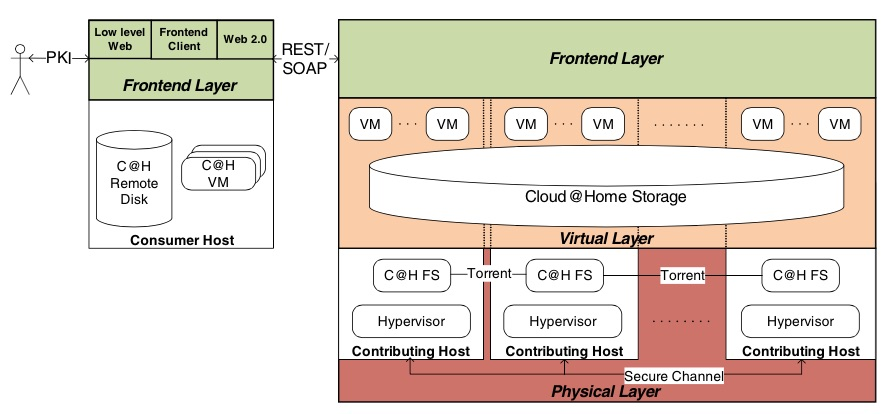
\includegraphics[width=125mm]{cathome_arch.jpg}
			\caption{Cloud@Home Architecture\label{cathome_arch}}
		\end{figure}
	\end{center}
	
	We can observe the three-tier approach to organize the architecture: \emph{Frontend Layer}, \emph{Virtual Layer} 
	and the \emph{Physical Layer}.
	\\
	The \textbf{Frontend Layer} is the realization of the answer to the \emph{Frontend} challenge 
	that they proposed in their preliminary discussion of the project. In order to achieve it, 
	they propose to split this layer into two parts, namely the \emph{Server-side} and \emph{Light 
	Client-side}. We can see that they adopt a client-server approach from the user's perspective, 
	and thus we can extrapolate that there is a hint for a centralized mean to deal with \emph{
	Resource Management} (as a matter of fact in a later paper, namely \cite{cathome6} and \cite{cathome9} 
	they explicitly express the need of a centralized entity w.r.t. Resource Management). 
	%% First difference, we attempt to propose a fully de-centralized cloud infrastructure....
	\\
	The \textbf{Virtual Layer} consist of a consequence to the \emph{Frontend} challenge, or in 
	other words \emph{How to provide homogeneous perspective of a set of heterogeneous resources?} 
	Their answer: through \textbf{Virtualization}, which enables us to discard the disparities within 
	the different hardware offered by the participants. This virtualization will take place into what 
	they call the \emph{Execution Service}, and the persistency of the data will be ensured by the \emph{
	Storage Service}. This service is analogous of the GoogleFS (file system) \cite{gfs}, which, in a nutshell 
	split files into \emph{chunks} of equal size, which are then distributed of different nodes called 
	\emph{Chunk Servers} (and replicated to ensure reliable storage). Finally there is a \emph{Master 
	Node} that catalogs all the meta-data about the data stored and simply indicate to the user which 
	Chunk Server(s) possess the parts consisting the file requested, thus the user retrieve the chunks 
	directly from the Chunk Server(s). This is a very naive simplification, but it serves to give an 
	overview how such distributed file system can be implemented (in the context of this Cloud 
	Infrastructure), and how from a user's perspective it resembles, as cited in \cite{cathome}:
	\emph{a locally mounted remote disk}.
	\\
	The \textbf{Physical Layer} act as the provider of physical resources to the layer above, but 
	also it encompasses all that is required to manage those resources (locally). Also they note that 
	it is here that the negotiation mechanisms, w.r.t. users contribution and request of resources,
	should reside and by trickling down from the precedent layers it's policies should be enforced.
	\\
	Finally this is a brief overview of the architecture that they propose for the Cloud@Home project, 
	but nonetheless sufficient for now. It provides the mainlines to start an analysis, and if required 
	we will in subsequent section to more specific aspect of this architecture as a mean of comparison 
	to the architecture that we propose for our proof of concept.
	
	\subsubsection{Brief Analysis}
	We've presented the biggest and most important project w.r.t. a large-scale Volunteer Cloud Computing 
	Infrastructure, now let's recapitulate the important points of this project. First they proposed to 
	a marriage between volunteer and commercially available resources, and on this basis develop a 
	business model that would give the ability to any user to monetize their volunteered resources. 
	Secondly, they proposed a 3-tier architecture that would answer the major challenges that they 
	identified, such as: offering a frontend that enables users to have a uniform homogeneous view 
	of the cloud infrastructure; segregate the resources according to two services (Execution/Storage);
	and how to manage resources and services within a distributed infrastructure. Finally, we can observe 
	that there is an intention of providing all types of delivery models: IaaS, PaaS, and SaaS.
	
	
	\subsection{P2P Cloud System}
	There was other notable effort conducted with respect to this concept, \cite{P2PCS}, albeit presented 
	under a different category one of Peer-to-peer Cloud Architecture. The authors propose and describes 
	the design and prototype implementation of a fully decentralized, P2P Cloud. They present the idea of 
	Peer-to-Peer Cloud Computing, which consist of building a cloud out of independent resources that are 
	opportunistically assembled. It could be built by assembling individual peers without any central 
	monitoring or coordination component. It would provide on-demand scalability, access to computing and 
	storage space with no single point of failure nor central management. Resources are added to the pool 
	of resources simply by installing a software daemon on them. Their proposed implementation is 
	advertised as a fully distributed IaaS Cloud infrastructure.
	\\
	They differentiate themselves from Cloud@Home by putting emphasis on the fact that it relies on centralized 
	components, while allowing users to contribute, (theoretically it isn?t required). Also, their architecture 
	is fully de-centralized and it doesn't require any central bookkeeping service. Finally, they note that there 
	is no known implementation to date of the Cloud@Home proposal.
	\\
	The System Model they propose consists of nodes, and these nodes join by installing a software daemon. 
	This software daemon presents two interfaces: a user interface and a node-to-node interface. The API 
	that is exposed by the user interface is similar to conventional IaaS Cloud APIs (such as Amazon EC2 or S3). 
	Nodes are managed by their respective owners in which case it offers no QoS guarantee. It goes for 
	applications failures/crashes; the responsibility is reverted to the users (as would be the case for 
	conventional IaaS Clouds).
	
	\subsubsection{Architecture}
	In this section we will briefly present the architecture of the P2PCS, and briefly analyze its 
	key features.
	 
		% need to find the picture of the architecture and replace this dummy jpg!!!!
	\begin{center}
		\begin{figure}[h]
			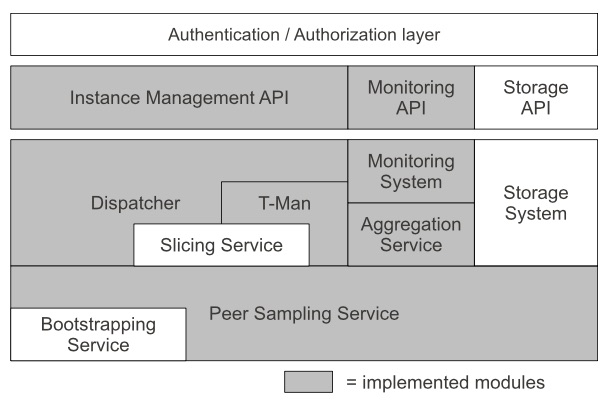
\includegraphics[width=125mm]{p2pcs_arch.jpg}
			\caption{P2P Cloud System Architecture\label{p2pcs_arch}}
		\end{figure}
	\end{center}
	
	We will briefly present each of the implemented modules (in gray).
	First the \textbf{Peer Sampling Service (PSS)} aims at providing each node with a list of peers to exchange 
	messages with. They achieve this by maintaining an unstructured overlay over the set of peers. It can 
	keep the overlay connected also in presence of churn, by using a simple gossip protocol. It uses a 
	BootStrapping Service to gather an initial set of nodes, although it not implemented yet; the current 
	implementation parses a text file with the IP addresses of the nodes.
	\\
	Second is the \textbf{Slicing Service (SS)}, which is used to rank the nodes according to one or more attributes, 
	it is also used to request slice of the whole cloud according to a user-defined criteria.
	\\
	Third is the \textbf{Aggregation Service (AS)}, which is used to compute global measures using local message 
	exchanges. It allows each peer to know system-wide parameters without the need to access a global registry.
	\\
	Fourth is the \textbf{Monitoring System}, which is implemented on top of the AS, and it collects global system 
	parameters and then provides them to the user. The MS API provides means to start and stop the display 
	of run-time instance informations. In the current implementation it is used to display the topology of 
	the network and the set of nodes of the slice a node belongs to.
	\\
	Fifth is the \textbf{T-Man component}, which is used to create a overlay network with a given topology, and it 
	is based on gossip protocols.
	\\
	Sixth is the \textbf{Dispatcher}, which is responsible for handling the requests submitted by the user through 
	the high level user interface and translate them into the appropriate low level gossip protocol 
	commands which are sent to the other nodes.
	\\
	Final is the \textbf{Instance Management API}, which contains all the functionalities to create and terminate 
	instances, and also to provide means to list which resources are held by this user.
	\\
	The implementation was done in Java, using the server-client paradigm.
	
	\subsubsection{Brief Analysis}
	It seems to be a dead project, since no updates were done or any changes were made since 2011. This 
	is one of the driving factors of this inquiry. Did support for this project stop out of disinterest 
	by the author, or did its tragic fate is the result of the coming to realization that it is not a 
	appropriate architecture for the Volunteer Cloud Infrastructure?
	
	The cornerstone of this architecture is the use of several gossip-based protocols to achieve such an 
	infrastructure. We need thus to analyze this design decision, in order to assess its effectiveness 
	with respect to particular problem that they are employed to solve.
	
	\section{Motivation}
	The motivation behind this proposal, is to analyze wherein lies (if any)
        the shortcomings of previous attempts with respect to the problem at
        hand. Thus we need to formally define the problem, then based on the
        analysis of these two proposal we will attempt to apply our conclusions
        in a proof of concept that demonstrate the feasibility of our
        solution. In this section we will present a formal definition of the
        problem we are addressing, followed by the justification of the
        assumptions and the major design decisions.

        \subsection{Problem Statement}
        The specific nature of the problem of creating a Volunteer-based Cloud
        Computing infrastructure, lies in the ability with which it aggregates,
        presents, utilizes, and deals with the intrinsic properties of
        collaborative distributed system. But we strictly focus on providing an
        analysis of a fully de-centralized type of architecture, in this case
        one that operates in an \emph{ad-hoc} manner, or using a peer-to-peer
        topology.  \\ Second portion of this problem statement is relative to
        the service model for which we choose to address, the
        Platform-as-a-Service. It is beyond the scope of this thesis to provide
        a full and comprehensive infrastructure that addresses the complete
        spectrum of service models. But it is important to note, the problems
        identified w.r.t. the challenges of collaborative distributed system are
        the same regardless of the service model, that this thesis could serve
        as a starting point towards the definition of this generalized Cloud
        Infrastructure. \\ By focusing on PaaS we need to provide a usable and
        unified API, in the likes of Google App Engine. Thus we need to discuss
        the requirements of such an API and try to address most of them using
        state of the art techniques and mechanisms. It is imperative to always
        keep the fully de-centralized perspective when analyzing the different
        parts of this problem. In other words how does the peer-to-peer topology
        affects the requirements, design and implementation of this API, compared to a
        centralized PaaS as provided by Google and Amazon. \\ Third portion of
        this problem is to answer, based on our conclusions, how well is the
        peer-to-peer topology, in the context of collaborative systems and
        Volunteer Cloud Computing, fares against commercially available
        solutions and what are the incentives (if any) to such a system.

	\subsection{Service Model}
	We need to situate where, within the already defined ontology of Cloud
        Computing, our effort will focus. This effort focuses on the
        Platform-as-a-Service model, conversely to \cite{cathome} which
        attempted to propose a solution for all of the service models, and
        conversely to \cite{P2PCS} that provides a solution w.r.t. the
        Infrastructure-as-a-Service model.  \\ The driving factor to focus on a
        PaaS model, is that we intend to propose a solution that does not
        require any Hypervisor, and thus this solution will operate using Light
        Virtualization (in the form of containers and more precisely groups
        \cite{cgroups}). Rather than providing an infrastructure on which
        different VM can be deployed, we want to abstract this infrastructure by
        simply providing an environment on which code can be executed,
        regardless of the underlying infrastructure.  \\ Although this
        implementation of the proof of concept targets the PaaS model, we will
        show at the end that the underlying infrastructure that has been
        developed can be used in the context of SaaS also.
	
	\subsection{Applications}
	The C@H project presents 
	
	\section{Contributions}
	In this section we will present our novel contributions with respect to previous related work.

        %--- May need to find a way to transition between these two
        %--- sections, what follows is the breakdown of the different
        %--- layers by analyzing the past effort, to culminate to the
        %--- presentation of our architecture.

	\section{Network Layer}
        Upon our literary review we have found a framework that
        focuses on identifying the challenges and characteristics of
        collaborative applications over peer-to-peer systems
        \cite{p2p_collab}. It proposes the following definition of a
        collaborative system:
        \begin{quote}
          [...] a P2P system that aggregates a group(s) of diverse resources to
          accomplish a greater task.
        \end{quote}
        It is important to point out the motivation of this paper is to
        characterize and formalize the P2P resource collaboration problem and to
        evaluate the current state of the art with respect to this
        characterization. They identified 7 key phases that characterizes this
        problem and we will present them briefly, for a more extensive
        definition please see \cite{p2p_collab}:

        \begin{enumerate}
          \item \textbf{Advertise}: Each node advertises its resources and their
            capabilities using one or more formal specification (Resource
            Specification) over a defined set of attributes.
          \item \textbf{Discover}: Nodes may use a mechanism to discover and
            keep track of the useful specification advertisements from the
            other participating nodes. This enables to accelerate the querying
            mechanisms but also to preserve inter-resource relationship
            information.
          \item \textbf{Select}: Provide mechanisms for an user to select a group(s)
            of resources, that satisfies a formal specification of his
            requirements, which contains attributes and ranges of acceptable
            values for these attributes.
          \item \textbf{Match}: Provide mechanisms to be able to formally
            specify inter-resource relationship requirements, to ensure that
            they satisfy the resource and application constraints, in the query.
          \item \textbf{Bind}: Provide a binding mechanism between the resources
            and the applications, to prevent that two application select the
            same resources. But also to cope with the dynamic nature of p2p,
            since a node may not be available at the time of use but was at the
            time of selection.
          \item \textbf{Use}: Utilize the best subset of available resources,
            from the resources acquired, to execute the application (and all its
            tasks) while respecting the constraints of both application and
            resources.
          \item \textbf{Release}: Provide a mechanism that allows to release
            resources in relation to the application demand, and/or the
            contractual binding (if time-sensitive). That mechanism can also
            provide means to partially release a resource to enable it
            collaborate with other applications.
        \end{enumerate}
        
        %--- need a quick transitional point (at least a reflection on
        %--- the qualitative properties of this framework). Need to express this caveat by
        %--- no means are any of these phases mutually exclusive, and the authors
        %--- acknowledge it. Some solution may group several of them into on component,
        %--- but still they represent the minimal set of IDEAL requirements for efficient
        %--- collaborative systems. We also need to point out the fact that they consider
        %--- two types of constraints, user-provided resource constraints and
        %--- application-centric constraints. 

        A fundamental concept of peer-to-peer systems, is the
        \textbf{Overlay Network}. It represents the superposition of
        two networks, one of which could be a physical network with
        physical connections, and the other a virtual
        network. Therefore, the overlay network represents a logical
        (or virtual) connection between nodes, and this enables to
        represent the absolute path between two nodes, in terms of the
        logical connection or virtual connection. As an example, if
        \textbf{Node A} is indirectly connected to \textbf{Node B} in
        the physical network architecture:

        \begin{center}
                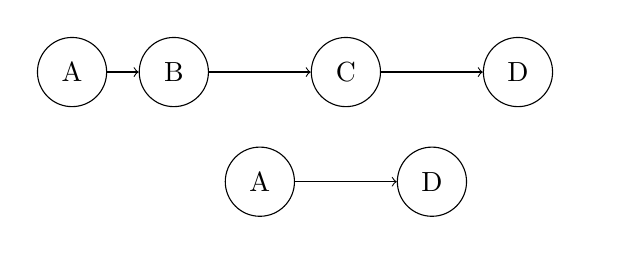
\begin{tikzpicture}[point/.style={circle,inner sep=0pt,minimum
                      size=2pt,fill=red}, skip loop/.style={to path={-- ++(0,#1)
                        -| (\tikztotarget)}}] 
                  
                  \matrix[row sep=5mm,column sep=2mm] {
                    
                    % First row: 
                    \node (A) [state] {A}; 
                    & & \node (B) [state] {B};
                    & & \node (C) [state] {C};
                    & & \node (D) [state] {D};
                    \\
                    
                    %Second row                                                                                                                                                                 
                    & & &\node (A2) [state] {A};
                    & &\node (D2) [state] {D};
                    & & &\\ };

                        \path  [->]  (A) edge node {} (B);
                        \path  [->]  (B) edge node {} (C);
                        \path  [->]  (C) edge node {} (D);
                        \path  [->]  (A2) edge node {} (D2);
                \end{tikzpicture}
        \end{center}


        A indirect connection between two nodes can be expressed in a overlay network as
        the direct connection between the two nodes, in this case A and D.

        Thus it simplifies and abstracts the specificities of the underlying network
        structure. One the Overlay Network protocols, based on TCP/IP is Distributed Hash
        Tables (DHTs), we will come back to this after the analysis.

        In the following subsection we will present an analysis of the networking
        capabilities of the two solutions in the scope of the proposed requirements.
	
        \subsection{P2PCS}
        The authors of this solution propose a \emph{fully de-centralized peer-to-peer
          infrastructure}, and we will try to identify the different key phases proposed
        in the framework although we need to consider the author's caveat about mutual
        exclusivity of the key phases.
        
        \\ Phase (1) and (2) {Advertise and Discover} are coupled together in the Peer
        Sampling Service. But are not exhaustively implemented, by this we underline the
        fact that they provide no mechanism to advertise the resources that a node offers
        to the network explicitly. Either using formal means, as proposed in
        \cite{p2p_collab}, or any other means, rather the PSS simply makes a node presence
        known to the other nodes via a simple gossip-protocol. This protocol grants a node
        with list of \emph{k} neighboring nodes, it consist of a \emph{local view} that
        represent the connections to this node \emph{\textbf{since}} the last message
        exchange (they refer to this concept of performing an exchange of message as a
        cycle) or cycle. Finally it provides a randomly structured graph, which is shown
        to stabilize under considerable amount of churn within a very short amount of
        cycles even with very pessimistic assumptions and no parameter tuning \cite{pss}.

        \\ Phase (3) {Select} is accomplished by the Slicing Service, although they admit
        that no implementation is provided at the moment of the writing of this
        paper. They based their design decision on the following paper
        \cite{jelasity2006ordered}, which presents a very clever algorithm. The problem
        that this algorithm attempts to solve, is referred as \emph{the ordered slicing
          problem}, which can be define as follows: \emph{generate a partitioning of nodes
          in a graph that centric to a given metric}. In this specific case, the graph
        represents the overlay network and the metric represents a desired property
        characterizing the application or resources constraints. The authors of
        \cite{jelasity2006ordered} assert that this algorithm is easily generalizable, and
        could be extend to deal with overlapping partitions (multi-attributes
        query). Finally, for analytical purposes it would have been interesting to see how
        the implementation of this algorithm w.r.t. multiple attributes would have behave
        with the complexity of the QoS that are necessary to a collaborative volunteer
        cloud infrastructure, rather than simply implementing it with a unique metric (the
        number of desired nodes).

        %--- Need to review the 2014 multi-dimensional paper to disprove the ability of
        %--- querying multi-attribute using this specific gossip-based protocol.
        
        Phase (4) {Match} is suspected to be realized, if ever, by the SS by a further
        specification of the query, but this is not clear within the slicing algorithm if
        it would be able to consider the inter-relations of the nodes in the slices,
        additionally to the set of queried attributes...

        Phase (5) {Bind} responsibility is accounted by the T-Man gossip-based protocol to
        build overlay networks with a given topology. It is accomplished by creating a
        distinct ring overlay of all the peers contained in a specific slice, 1 ring per
        slice. Thus slices are mutually exclusive. From this perspective, it seems to
        enforce a good binding policy. Although the question of concurrency, in the
        context of initially binding the resources to an application rather than another
        that requests the same resources, is completely left-out. It is a crucial
        question, since the slices are generated with respect to a metric (composite or
        unique) which ensures the application's constraints w.r.t. to the QoS. We can
        quickly observe the fact that the slices may become inadequate if one of (major
        contributing) resource are lost in a concurrent binding attempt between two
        \emph{"competing"} applications. Finally, we can conclude that by implementing the
        slicing mechanism using a single attribute, namely the number of requested nodes,
        there is no eminent concurrent binding problem because that it would only occur in
        a very specific case. It would manifest in the form of two or more concurrent
        requests for which the total requested number of node combined, would exceed the
        total number of available nodes, but the number of requested node per request
        would be inferior to the total available nodes. The problem ultimately becomes
        which application is entitled to have their request fulfilled, with no a priori
        any ranking mechanism (or reputation mechanism) to draw a fair conclusion?

        Phase (6) {Use} can be interpreted as being manifested by the Dispatcher, which
        translates the higher-lever API requests into the appropriate low-level gossip
        protocol commands which are sent to the other nodes. (Not fully clear as to how it
        manages to accomplish that???)

        Phase (7) {Release} would be accomplished by the Instance Management API, that
        grant the ability to the user to control the instances it harvests. BUT they
        express no means of automating the scaling of the resources it possess to respond
        to the increase of demand or the decrease of the demand. We could extrapolate that
        the Monitoring System in conjunction with the Aggregation Service could provide
        enough information to implement such functionality, but nonetheless they fail to
        make the point.

        \subsection{Cloud@Home}
        A majority of phases are somehow accomplished by the Management Subsystem. In
        \cite{cunsolo2010open}, there is two important passages that reflect their
        ideology with respect to the design adopted:

        \begin{quote}
          In order to enroll and manage the distributed resources and services of a Cloud,
          providing a unique point of access for them, it is necessary to adopt a
          centralized approach that is implemented by the management subsystem.
        \end{quote}

        \begin{quote}
          The management subsystem is implemented as a centralized subsystem managing the
          whole infrastructure. Although this solution introduces a single point of
          failure into the architecture, this is the only possible way to manage resource
          QoS, SLA, dynamic provisioning, and monitoring because there has to be a
          subsystem that aggregates information and has to know the condition of the whole
          infrastructure, there needs to be a coordinator. Reliability, availability, and
          fault-tolerance issues can be achieved by replicating the management subsystem
          and its components, adequately managing the consistency of redundant replicas.
        \end{quote}

        \\ In the first quote they assert the need of a centralized entity to accomplish
        the three key phases: Advertise, Discover, Select, and arguably Match/Bind. This
        is where we want to verify this kind of assertion, since the previous attempt
        P2PCS, seems to point in the opposite direction.  
        
        \\ The following quote is interesting because the admit the creation of a single
        point of failure, by consequence of this design decision. Furthermore, they assert
        that any other type of infrastructure (by design) is inherently inadequate to
        manage resource QoS, Service-Level Agreements, dynamic provisioning, and
        monitoring. Their validating argument is the need of an aggregating service that
        possesses knowledge of the state of the infrastructure as a whole, which is
        debatable and definitely needs justification for the introduction of a centralized
        entity, in the context of peer-to-peer systems. Thus, one can deduce from this
        line of thought that Cloud@Home argue the need for a centralized entity as a
        solution to these key phases: Advertise, Discover, Select, Match (partially) and
        Release.
        
        The Management Subsystem is given the task to collect the user's request to
        assimilate and provide them in the proper format to the corresponding
        subsystem. The Resource Subsystem is responsible for the resource management, thus
        it receive a translated request from the Management Subsystem and it is
        responsible to look through its collection of resources and find the most
        appropriate selection of resources that satisfies this request. It operates in
        hierarchical fashion using Schedulers and cluster-type groupings, with a very
        elaborate load-balancing policy that is extensively described in
        \cite{cathome9}. Finally, one can conclude that the Resource Subsystem is
        responsible for the following phases: Match (partially), Bind, and Use.

        \subsection{Musings}
        From these analyses we can draw some conclusions, but more importantly lay out the
        different point of views that we need to address within our own architecture. The
        first point of view that seem to emanate from the P2PCS project,
        \emph{gossip-based protocols are centric to this peer-to-peer collaborative
          system}, which give rise to the following question:
        
        \\ \emph{Are gossip-based protocols the most adequate technology to fashion a
          collaborative peer-to-peer infrastructure?}

        \\ The second point of view that is of interest, originates from the Cloud@Home
        project, and give root to this line of interrogation:
        
        \\ \emph{To which extent is the need for centralization, with respect to
          management of QoS and SLA, dynamic provisioning and monitoring; is accurate in
          the context of the collaborative peer-to-peer infrastructure? And if provably
          accurate, is the design for P2PCS fundamentally flawed, do we need to divert our
          attention to more sensible solution?}  

        \\ These interrogations will be the driving inquiry factors to the elaboration of
        our architecture, which we will attempt to resolve before presenting it. Thus, the
        following subsections will deal with providing a rationalization of these line of
        thoughts.

        \subsection{Gossip-based protocols, what is the chat about?}
        Peer-to-peer systems implements an overlay network, which can be categorized into
        two broad categories, with respect to their structure and are defined as follows
        \cite{lua2005survey}:
        \begin{enumerate}
          
          \item \textbf{Unstructured Networks}:
            \begin{itemize}
              \item Peer organization results in a random graph, which is in a flat or
                hierarchical topology.
              \item Querying is generally done using flooding or random walks.
              \item Locality is not preserved relatively to the topology and the data.
              \item Supports complex queries.
              \item Non-deterministic queries.
            \end{itemize}
          \item \textbf{Structured Networks}:
            \begin{itemize}
              \item Peer organization results in a structured graph, consisting of
                dividing the responsibility of the key space among the peers.
              \item Keys are mapped to a unique live peer, and are assigned to data
                objects via different means, hashing being the most popular.
              \item Locality is generally preserved.
              \item Provides efficient mechanism to query data objects using keys, in the
                order of $O(log n)$.
              \item Does not support complex queries.
              \item Queries are deterministic.
            \end{itemize}
        \end{enumerate}
        Gossip-based protocols, or epidemic protocols, falls generally into the
        Unstructured Networks category, with the exceptions of gossip-based protocols like
        T-Man which focuses on generating a structured overlay network
        \cite{jelasity2009t}. First practical representation of epidemic algorithms in the
        context of computer science is attributable to \cite{demers1987epidemic}. Since
        then, the gossip/epidemic protocols have had several praises and criticism, which
        led to some skepticism w.r.t. it's relevance. Lately a revival of the idea of
        gossiping protocols emerged, mainly because of the extensive body of work done by
        Mark Jelasity from the University of Szeged, in Hungary; with respect to its
        applicability in large-scale distributed networks. A gossiping framework was
        defined, in \cite{riviere2011gossip}, to circumscribe and represent the various
        gossiping protocols. Where each node in the system maintains a partial local view
        of the system, where the partiality is intrinsic to the system size. Interactions
        within the system consist of pair-wise periodic exchanges of information among
        randomly selected peers, resulting is eventual correctness of each partial
        view. The strength of this approach lies in property to achieve local
        convergence, as driving factor for the nodes decisions, will result to global (or
        system-wide) convergence. More specifically it provides, as emergent properties of
        the quantity of interactions involved, a self-stabilization, self-healing and
        self-configuration characteristics. All of these properties are dependent of
        convergence criterion, be it local or global.

        \\
        Epidemic protocols, promises a lot of very interesting properties, lets refer back
        to \cite{p2p_collab} to make sense of these properties in the collaborative
        peer-to-peer system context. They make several interesting observations about
        Unstructured Networks compared to Structured Networks, here's a list of those that
        we did not already addressed:
        \begin{enumerate}
          \item \textbf{Overhead Maintenance}: is relatively low in the case of
            Unstructured Networks, and moderate in the case of Structured Networks.
          \item \textbf{Failure/Churn Resistance}: is high in the case of Unstructured
            Networks, and moderate in the case of Structured Networks.
        \end{enumerate}
        Thus given the previous observations, and the present one, we could argue the
        following: Unstructured Networks provides a mean achieve connectivity in highly
        dynamic environment, thus are robust and resilient to failures. Also they provide
        querying mechanism that support complex queries, but answer those queries in a
        non-deterministic manner or as it is often referred as best-effort. Finally, it
        has unpredictable boundaries on time complexity, thus it is requires to define a
        maximum on the number of hops, which corresponds to the number of nodes traversed
        during the walk through the graph and acts as a bound on time complexity. The
        majority of Unstructured Networks are implemented via gossiping-protocols,
        although it was proven a very fast and efficient mean to construct overlay
        topologies that are structured \cite{jelasity2009t}. Structured Networks, provide
        a structural organization of the nodes and the data (in the case of DHTs) which
        generally preserves locality. It provides a efficient querying mechanism, which is
        advertised to operate within a $O(log n)$ time complexity (although
        \cite{bandara2012evaluation} showed that this complexity was theoretical, and that
        in practice it is more in the order of $O(n)$).
        
        \subsection{To structure or not to, that is the question}
        Two of the primary distinctive advantages to using Unstructured Network over
        Structured Network, are summarized as follows: The ability to generate complex
        multi-attribute queries and the resilience over very high presence of churn. Thus,
        we need to understand to which extent these are required in the context of
        Volunteer Cloud Computing. 
        
        \\ If we refer to the current Volunteer Computing efforts, such as the @HOME
        paradigm, we quickly realize that they use a centralized infrastructure and it has
        some advantages. One of those is to keep a centralized repository of the host,
        which provide enough contextual information to quickly restart a failing
        host. Also, and most importantly this does not require, from the host(s)
        perspective to preserve any contextual knowledge or structural knowledge of the
        other nodes from a graph's perspective. This reduce the problem, for the host, to
        simply reconnect to the centralized node (thus it is only required to know one IP
        address (of the server)).And we can then notice that Cloud@Home does emulate this
        notion of a central managing entity, thus it remains true to the @Home
        paradigm. In our context, since we are aiming at a fully de-centralized
        architecture, we need to take into account the structure of the network since we
        do not wish to introduce a centralized entity. This entails the consideration of
        the dynamism of the underlying infrastructure in the context of collaborative
        applications, as was the case with P2PCS. 

        \\ Given the analysis of the P2PCS, which leads us to believe that the dynamism of
        the network with respect to peer to peer systems, unstructured networks appears
        the most adequate. Adequacy, in this case, can really be defined given the two
        advantages presented with unstructured networks. First, it is more resilient in
        presence of very high churn rate. But can we sacrifice resilience and achieve an
        acceptable network layer architecture, that satisfies complex multi-attribute
        queries? Therefore we need to draw the line, and identify typical queries that are
        necessary in the context of volunteer cloud computing. Because, it is important to
        distinguish between general collaborative system requirements, and our specific
        requirements for our application. It can reformulated as the following: \emph{What
          are the requirements for slicing w.r.t. Volunteer Cloud Computing?} or
        \emph{What are the minimal requirements for the specification of the resources,
          that will provide a adequate domain for queries in the context of VCC?}

        \\ Slicing is a concept that applies to distributed systems and is concern with
        the partition of a large set of node in a given graph with respect to attributes
        (metrics) that are local to the nodes. Thus, complex multi-attribute queries can
        be represented as a slicing problem for which given a set of attributes (or
        metrics), with fixed values or ranges of values, what is the optimal partition of
        nodes that correspond to this query (with respect to the set of requirements that
        are formally defined by this set of attributes). As stated above, gossip-based
        protocols provide means to execute complex multi-attribute queries, as shown in
        \cite{pasquet2014autonomous}. This favor the use of Unstructured Networks, but
        simple multi-attributes queries can be performed on Structured Networks given that
        they use a proper structure, as identified in \cite{p2p_collab}. They show three
        very simplistic version of a ring-structured overlay:
        \begin{enumarate}
          \item Separate overlays for each attribute, then depending on the query: choose
            the appropriate overlay and resolve it. Although, in this case the query are
            single-attribute, it provides means to query different attributes
            independently.
          \item Partition the overlay in such a way that it distributes the nodes relative
            to the pre-defined attributes. Thus, nodes that possess similar attribute
            values will be closer on the ring. It provides a mean to resolve a
            multi-attribute query as multiple sub-queries.
          \item Overlay with overlapped attribute space, such that the position of a node
            is dictated by the juxtaposition of its attribute values in the
            key-space. This does not allow to resolve multi-attribute queries directly,
            rather it allows to resolve single-attribute queries that are the product of
            multi-attributes juxtaposition.
        \end{enumerate}
        The comparison that they have done shows that current Structured Network solutions
        are analogous to a tablecloth that is too short. No matter which way you pull on
        it, which perspective you take to provide a solution, it will uncover another part
        of the table, thus providing a solution to a specific problem will in turn shed
        light onto other problems with respect to peer-to-peer systems. One concrete
        example that they provide is one of MURK \cite{ganesan2004one}, which propose to
        model the attribute space as a d-dimensional torus, where each dimension is
        representative of specific type of attribute. To deal with the sparsity of the 
        attributes composing real-world queries, since in the initial proposition this
        results in multiple dimensions that are ignored (or irrelevant), they showed that
        it could be mapped to a Chord ring and thus reducing the
        dimensionality. Nonetheless, it results in a lost of locality, given a large
        dimensionality, and the query resolution cost is now bounded by $O(n)$ with the
        newly introduced overhead.
        
        \\ We obviously see that it is impractical to use a Structured Network, especially
        a ring-based one, to solve the Slicing Problem that is present in distributed
        systems. Also, that an Unstructured Network lacks the ability to resolve queries
        in a deterministic manner but provides a decent solution to the Slicing Problem
        and is more resilient to churn. This is an open problem in distributed systems
        even though it seems to point towards Gossip-Based Protocol as being the solution.
        % point out some limitations of Gossip Based protocols... from this paper: The
        % promise, and limitations, of gossip protocols For this thesis, and due to its
        scope, we intend only to underline it and present some of the current
        trends. Thus, to produce a workable proof of concept, we require determinism and
        single-attribute query will suffice, we will use a DHT named Kademlia. In the
        following subsection we will quickly present Kademlia, simply to provide a more
        technical understanding of our Network Layer.

        \subsection{Kademlia}
        Proposed in 2002 \cite{maymounkov2002kademlia}, Kademlia is a Distributed Hash
        Table that was designed for peer-to-peer networks. In this DHT, the nodes are
        assigned 160-bit identifiers, producing a key space of $2^160$, and its lookup
        algorithm uses a XOR metric topology to locate the nodes in a logarithmic time
        complexity. More specifically, since the keys and the node ID's are of the same
        length and type, using a simple exclusive-OR between the two results in an integer
        representing the distance of the key (for which we are searching) and the current
        node. Also, as a consequence of using such a metric for distance, three properties
        emerges:
        \begin{enumerate}
          \item \textbf{Triangular Inequality:} given node: A,B,C,  $dist(A,B) \leq dist(A,C) + dist(C,B)$
          \item \textbf{Symmetric:} $dist(A,B)=dist(B,A)$
          \item \textbf{Distance from/between itself:} $dist(A,A)=0$
        \end{enumerate}
        It was shown by the creators, that each lookup iteration reduces the distance from
        the key (for which we are searching) by one bit, and thus a search for a key among
        $2^n$ nodes ranges from 1 to $n$ lookup iterations (best case to worst
        case). Thus, given it simplicity, its determinism and its popularity (\emph{being
          used by eMule community as a successor to their previous network infrastructure,
          also by BitTorrent, Osiris SPS, and Gnutella to name a few)}; we decided that it
        would make an ideal candidate for our proof of concept.

        \section{Virtual Layer}
        In this section we will describe the next layer in our infrastructure, the Virtual
        Layer. Its responsibility is to provide means to make resources homogeneous to the
        end user. By this we mean that it is responsible to provide a level of abstraction
        from the specificities of each physical machine (resources). If we quickly review
        how this is accomplish in Cloud@Home, we notice that they propose using Virtual
        Machines and Hypervisors to manage them. We can rationalize this idea since they
        intend to offer a full-fledged Cloud Infrastructure covering the three major
        services models, and to make it efficient it is necessary to be able to treat each
        machine (or contributor) as one that can "spin" a VM (whatever it may be). On the
        other hand, P2PCS took the same perspective, but they are only offering IaaS,
        rather than the three service models. And there are some advantages in doing so,
        first it removes the difficulty of deploying on different architectures, since by
        using this type of virtualization it resides on the application-level. Also it
        provides the ability to be OS or platform agnostic, because on a Windows machine,
        it is possible to run a VM with Linux as an OS, and vice-versa. We propose to use
        a different type of virtualization, namely Light-Virtualization.
        
        \subsection{Light Virtualization}
        Light Virtualization, also referred to as \emph{Containers}, comes in different
        flavors, such as LXC, Solaris Containers, OpenVZ, and FreeBSD Jails, the
        differentiation from full virtualization, is best described with the following
        picture \cite{dell}:
        \begin{center}
                \begin{figure}[h]
                        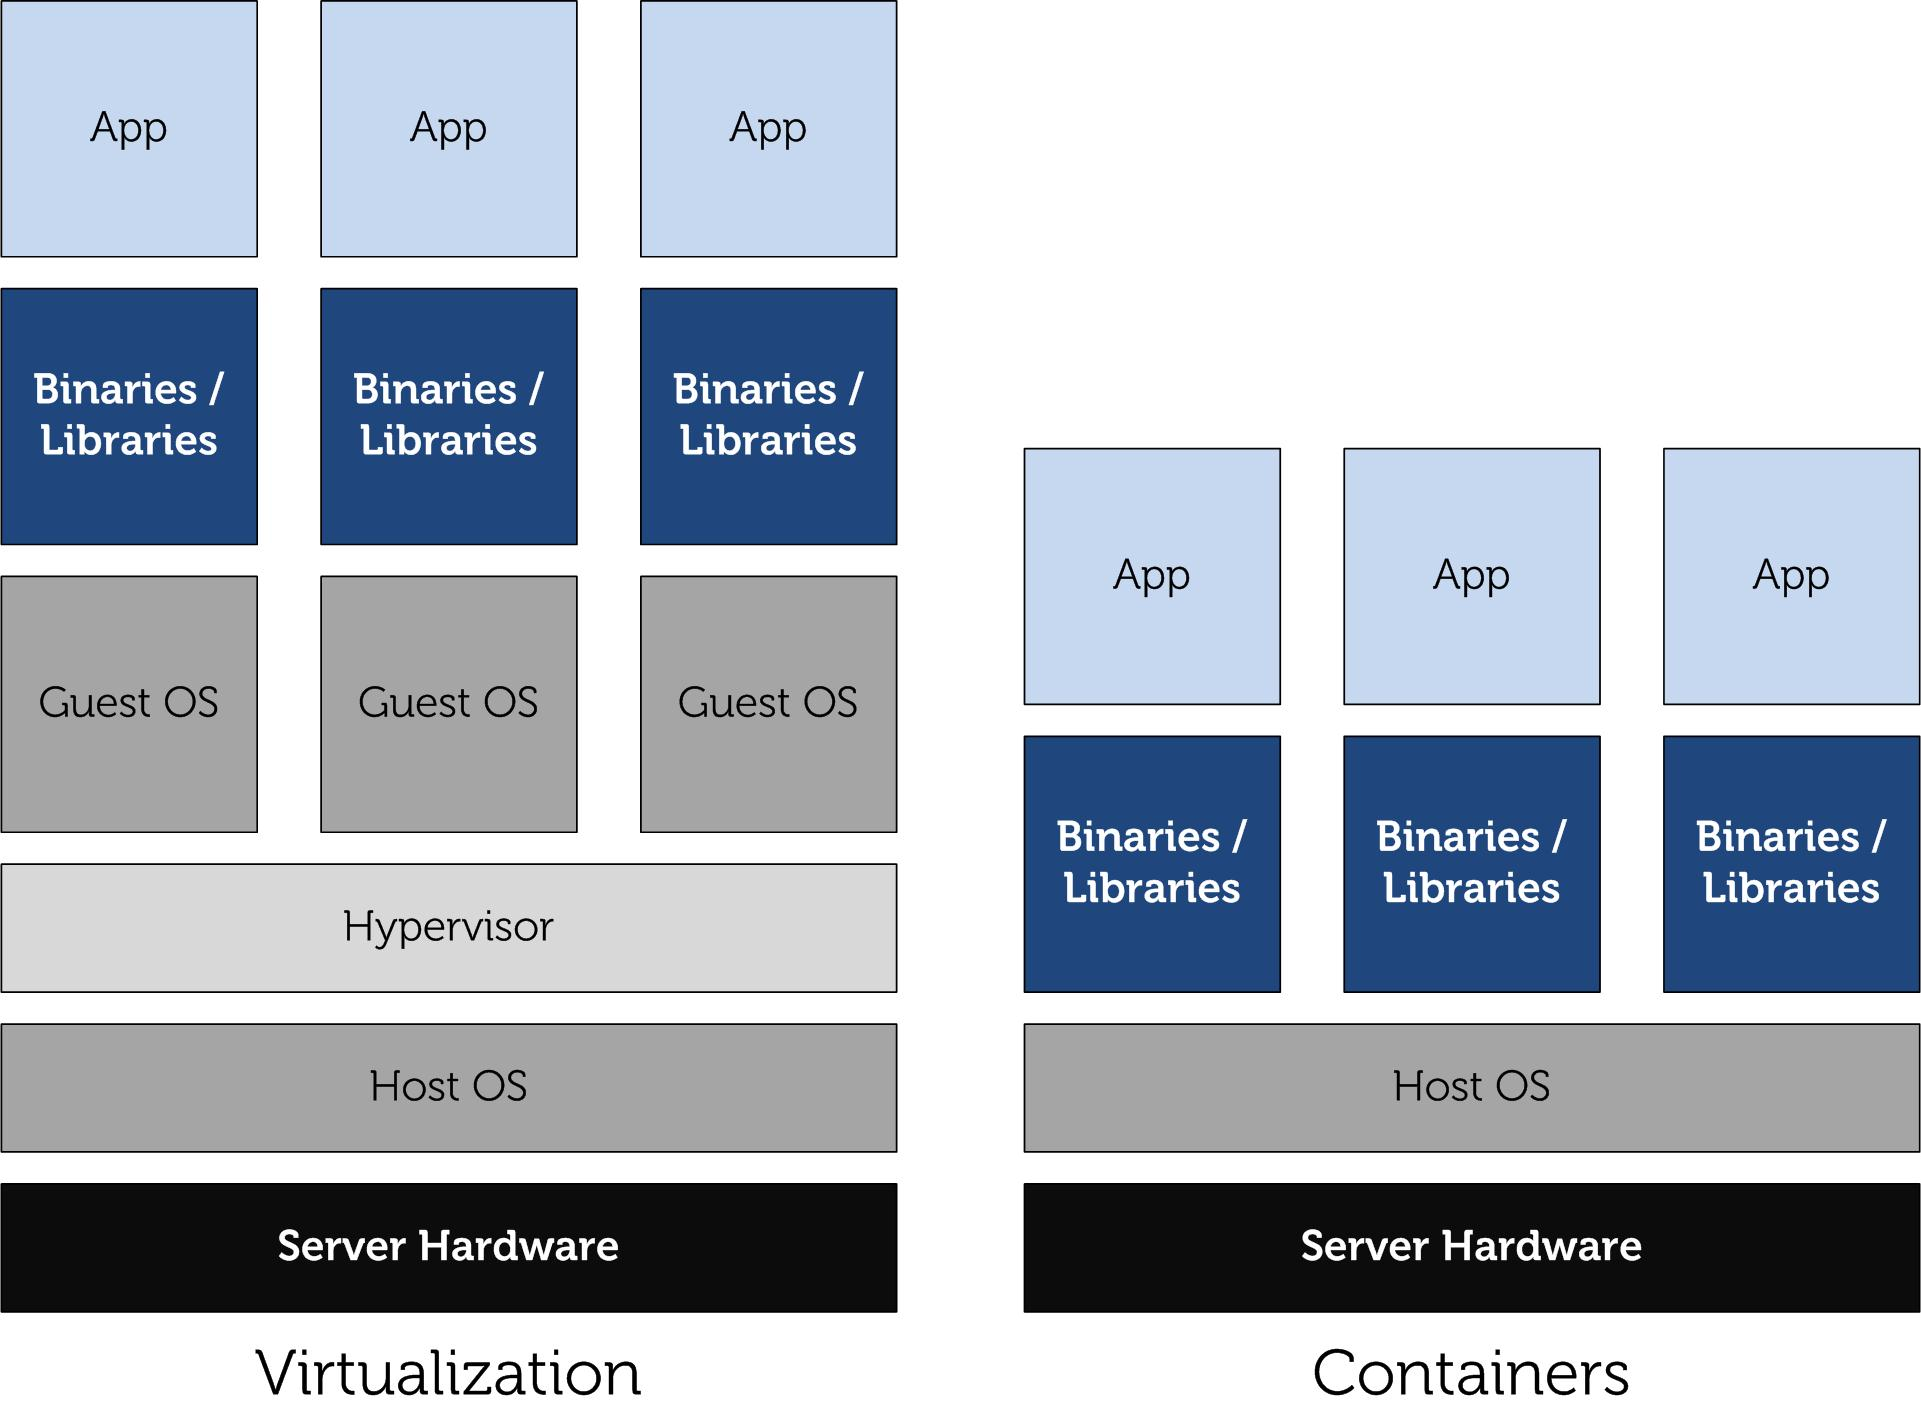
\includegraphics[width=125mm]{lxc-vm.jpg}
                        \caption{VM vs. Containers\label{vm_containers}}
                \end{figure}
        \end{center}
        We can notice that footprint of traditional virtualization is greater, since it
        requires a Hypervisor to monitor and manage each instances (or VMs) that are
        executed on this single machine (be it server or personal computer). Whereas the
        footprint of Containers is less, since it requires no intermediary entity control
        the instances running on this single machine, but even more important, each
        instance does not requires to run its own OS. Rather it shares the same Kernel,
        and simply segregates the resources into logical units (or instances). This
        results in a boot time that approaches mere seconds, rather than just shy of a
        minute to fully boot a complete operating systems. And this leads to the final
        important differentiation, how the physical resources are used? In the case of
        traditional virtualization, the resources are divided and allocated to each VM
        exclusively; whereas using light virtualization the resources are shared by every
        containers (although they can be restrained to a certain usage
        boundary). Although, given this hypothetical situation where one is required to
        run several instances of the same OS (cluster creation), using traditional
        virtualization it would still require a Hypervisor and a complete version of the
        (same) OS running on top of the host OS. But using Containers cluster creation is
        easily achievable and only requires one single Kernel to be executed on the
        physical machine.

        \\ All of this is possible due to a conceptual construct called \emph{c-groups},
        in Linux, or control groups. It was defined as a Kernel patch in
        \cite{cgroups}, and consists of an aggregation and partition mechanism for
        groups of task (or sets), that contains (within those partitions/aggregations) all
        their future children. It generates a hierarchy of groups, for which different
        specialized behaviors can be explicitly defined. The authors admits that in its
        own, cgroups provides only tracking capabilities for simple jobs. But used with
        other subsystems (such as cpuset) it can provide additional properties for the
        groups of processes (i.e.: restraining the execution of a group to a specific
        CPU-core).
        
        \\ As an example of these emergent properties, LxC (Linux Containers)
        leverages cgroups to achieve resource isolation and namespace isolation without
        ever needing any virtual machines. Namespace isolation, grants the ability to
        isolate running applications completely from the operating system environment such
        that two applications running into two distinct namespace, albeit not an exclusive
        feature of LxC. A general example of namespace isolation is the \emph{PID
          namespace} \cite{emelyanov2007pid}, which grants the ability to create sets of
          tasks such that each set is completely independent from one another. Thus, two
          processes belonging to different sets of tasks, can have the exact same ID,
          without any ambiguity since they do not belong to the same set. 

          \\ Another interesting contender in the container's scene, is the ever popular
          Docker. Released on March 2013, this software is only around a year and half old,
          and it already has its own convention, DockerCon \cite{dockercon}, and is endorsed
          by major technological companies such as IBM, and RedHat (to name a few). Docker
          is open-source and provides means to automate deployment of applications within
          containers. Thus, it provides a higher-level interface to containers, by
          abstracting the intricacies and specificities into an intuitive and easy to use
          high-level API. This is the reason that we will use Docker for our virtualization
          needs in our proof of concept, since it provides a simpler interface, but it
          should be noted that using LxC would be recommended for a more complete
          implementation. Because it is not needed to provided this level of abstraction for
          our Cloud Computing Infrastructure, and it would be beneficial for less powerful
          machines not having to provide this which would result in a diminution of the
          overhead.

          \\ From a Platform-as-a-Service model point of view, this kind of technology
          solves a lot of important issues that rises from using a heterogeneous set of
          resources. As far as we are concerned, from our literary review, we are the first
          to propose the use of containers (or Light Virtualization), in the context of
          Cloud Computing, as a mean to provide physical virtualization of the
          resources. In the following subsection we will present Docker and its
          characteristics.

          \subsection{Docker}
          As presented above, Docker provides a high-level abstraction API to manage,
          configure, and monitor software containers. As a consequence, it augments
          flexibility and portability of the applications contained, since it is fully
          self-contained (it provide means to package the application and all of its
          dependencies). This is why we opted to use it as our virtualization software,
          because we could deploy totally self-contained applications in a very intuitive
          fashion. Thus we will provide a more complete overview and showcase why, as a
          prototyping tool, Docker is a excellent candidate.
          
          \subsubsection{Overview}
          It makes use of several different technologies, such as \emph{Namespaces} and
          \emph{Control Groups} to provide isolation from the host operating system
          environment and resulting in a self-containing property. Also, it uses Union
          File Systems, which are used to provide fundamental building components to the
          containers. UnionFS is a Unix filesystem service that provides means for virtual
          file systems to be created from separate file systems, using different branches
          (layers) per file system to represent the files and directories. Thus overlaying
          all the branches provides a single view of the multiple file systems, hence the
          name Unification File System. Docker utilize this for its images technology to
          provide lightweight versions (or simply the difference between the base image)
          of a Linux OS image. 
         
          \\ It uses a client-server model, for which the server is referred to as
          \emph{The Docker Daemon}. The client and server can be on the same host, but is
          not required to (which enables us to have a very light client on the nodes and
          we could have a central node acting as a server). All the most intensive task
          such as building the container, running it and/or distributing it is performed
          by the server, which is really neat since we can offload it to more powerful
          machines and keep the clients to a minimal performance
          requirement. Communication between the client and server can be done through
          sockets, or using a RESTful API (which again is a very nice feature for
          distributed application or environment).

          \\ We need to introduce three fundamental constructs of Docker to understand how
          it works. First is the construct that pertains to building containers, namely
          \emph{The Docker Images}, which are read-only templates from which containers
          are built. Subsequently is the distribution construct, or \emph{The Docker
            Registry}, which are private or public repositories that indexes and stores
          images. Finally, the construct that pertains to running applications, \emph{The
            Docker Containers}, which are analogous to directories in a file system. It
          contains everything that is required to execute the application it contains,
          thus there is no external dependencies. Created from Docker Images, a series of
          different commands can be executed on the containers, such as: run, start/stop,
          move and delete. In other words a Docker containers are created from Docker
          Images, which can be retrieved from public or private repositories referred to
          as Docker Registry or simply created from scratch. The resulting containers are
          completely self-contained and it is possible to interact with them using the API
          provided. Since it uses the UnionFS technology, when updating a container
          (really we are updating the image that represents this container) it is only
          necessary to provide the differences between the current image and the updated
          image, and this is done automatically. As a result the updates are small and
          fast. For our purposes, we use Docker to provide resource isolation, automated
          deployment, fast prototyping, means to automate container management and
          more. Finally, we still believe that since the we use containers as a
          virtualization device that enables us to utilize heterogeneous resources in an
          homogeneous fashion and once defined the images of the containers would remain
          the same, other than providing fast prototyping we would rather use a
          lower-level container technology such as LxC, which also provides means to
          distribute and manage application containers.
          
          \\ In the next section we will discuss our API layer design, and its
          features. Consequently we will proceed to present the challenges and open
          problems that are central to the API-level in the context of Cloud Computing. 
         
          \section{Application Program Interface Layer}
          APIs are generally used to express the contained components of a software
          (library) in terms of their functionalities, while expressing the expected
          inputs and expected outputs respectively. Usually the functionalities expressed
          are defined independently of their implementation, guaranteeing coherence and
          consistence from the user's perspective. Therefore this layer, in the context of
          Cloud Computing, will provide a set of building blocks to the application
          developer to utilize this Volunteer (or collaborative) infrastructure. In order
          to design an API that is well rounded, we've proceed to gather the requirements of
          an hypothetical PaaS API (platform) by observing how the different major service providers are
          implementing their own API and what functionalities are they providing. 
          
          \subsection{Requirements Analysis PaaS APIs}
          We are going to analyze two popular PaaS Service Provider's API, namely
          Google App Engine and Amazon Web Services. In order to do so we will attempt to
          reconstruct the requirements from the implementation and finally generate a
          specification of a hypothetical PaaS API platform. 

          \\ First we look at Google App Engine, \cite{gae_web},
          \cite{zahariev2009google}, and we should use the functional classification of
          the features offered (as presented in \cite{gae_web}) since there provide a
          total of 40 features. 
          \begin{itemize}
            \item \textbf{Languages and Runtimes:} it offers support for up to 4 different
              languages and recently added the ability to utilize Managed VMs (which
              allows to host on proprietary VM and grants more flexibility).
            \item \textbf{Data Storage, Retrieval, and Search:} it offers a plethora of
              DBMS (NoSQL, SQL, Blobstore) and storage mechanisms (Memcached, Logs), as
              well as access to Google proprietary searching mechanism via various APIs.
            \item \textbf{Communication:} it offers various mechanisms to ensure
              communication between user and host (Sockets, ChannelAPI, Twillio) and
              various protocols (Google Cloud Endpoints, XMPP).
            \item \textbf{Process Management:} it offers different task related queuing,
              monitoring and management related mechanisms.
            \item \textbf{Computations:} it offers a mean to manipulate images via its own
              Images API; also it offers full MapReduce integration and support.
            \item \textbf{Application Configuration and Management:} it offers a wide
              selection of analytics tools relative to the app (within the Google App's
              ecosystem), also offers various components to perform authentication,
              permit multitenancy, and testing related tasks.
          \end{itemize}
          It is important to note that GAE is a mature PaaS provider, and thus it explains
          the breadth of the components/features landscape. Starting from scratch we need
          to be able to differentiate which features or components are a fundamental
          construct of the platform, and only proceed to implement those. Although, if
          this project would be implemented not as a proof of concept, but a product aimed
          at a public release, we would eventually end up implementing many of those
          non-essential features. Rather than proceeding with an analysis of these
          features and cherry-pick a few essential ones, we will present the second PaaS
          API, namely Amazon Web Services, and this would provide (at least theoretically a
          less biased point of view with respect to proprietary technologies/infrastructures).
          
          \\ In the case of AWS \cite{AWS}, they use a similar functional classification but still it
          is somewhat different than GAE. Thus lets proceed to present the list:
          \begin{itemize}
          \item \textbf{Compute:} it offers automatic scaling, load balancing, and various
            other hardware/software inter-relational capabilities.
          \item \textbf{Storage, Content Delivery, and Databases:} it offers DBMS (NoSQL,
            Relational), different type of storage capabilities and content delivery mechanisms.
          \item \textbf{Networking:} it offers varying capabilities concerning networking
            related configurations (Virtual Private Cloud, DNS, dedicated connections).
          \item \textbf{Administration and Security:} it offers authentication mechanisms,
            access control, resource monitoring, logging mechanisms and cryptographic key
            management capabilities.
          \item \textbf{Analytics:} it offers real-time data processing, data warehousing,
            data pipelines as well as full Hadoop support. 
          \item \textbf{Application Services:} it offers queuing mechanisms, transcoding
            mechanisms, e-mail services, as well as search services.
          \item \textbf{Deployment and Management:} it offers various tools and services
            pertaining to application deployment, dev/ops resources management,
            integration tools and workflow related services.
          \item \textbf{Mobile and Devices:} it offers a series of tools and services that
            are aimed at facilitating compliance with various heterogeneous devices.
          \end{itemize}

          Although, some of these classes of services/features overlaps with the taxonomy
          of the GAE classification, some are completely unique (such as Mobile and
          Devices). From this array of different features and services we have devised the
          following taxonomy, represented by this graphic:          
          \begin{center}
              \tikzstyle{every node}=[draw=black,thick,anchor=west]
              \tikzstyle{selected}=[draw=red,fill=red!30]
              \tikzstyle{optional}=[dashed,fill=gray!50]
              \begin{tikzpicture}[%
                  grow via three points={one child at (0.5,-0.7) and two children at (0.5,-0.7) and
                    (0.5,-1.4)}, edge from parent path={(\tikzparentnode.south) |-
                    (\tikzchildnode.west)}] 
                \node {API Layer} 
                child { node {Databases/Storages}} 
                child { node {Front-End}} 
                child { node [optional]{Load Balancing \& Scaling}} 
                child { node {Security}} 
                child { node [optional]{App. Deployment and Management}};
              \end{tikzpicture}
          \end{center}
          For each of these components we will provide a brief defining characterization,
          and proceed to define our "barebone" API platform.
          \begin{itemize}
            \item \textbf{Databases/Storage:} it ensures the persistence of the
              information, and manages all data requirements within the application.
            \item \textbf{Communication and Networking:} it encompasses everything
              relating to web availability and connectivity, from web hosting (DNS related
              concerns: multiple IP addresses) to presentation (HTML/CSS and other
              presentation technologies) and also everything related to the end user via
              the frontend (REST/SOAP/Sockets).
            \item \textbf{Process Management:} includes the
              components to provide scalability (parallel software design, multitenancy) and
              load balancing (ensure even distribution of the workload).
            \item \textbf{Security:} it ensures secure communications (via encryption and
              decryption), access control of data and/or resources, proper authentication
              and as an emergent characteristic enables coherent and consistent
              multitenancy. 
            \item \textbf{App Deployment and Management:} provides capabilities to the
              deployer to manage and monitor resources (usage and performance), and
              provides various analytic oriented tools 
          \end{itemize}
          Based on this we will present an overview of the possible way to achieve these
          different functional requirements by means of literature review. Thus we will
          present an accurate picture of where the state of the art lies concerning the
          specific problems that are inherent to each of these requirements.
         
          \subsection{Databases and Storage Solutions}
          As we have observed in GAE and AWS, they provide a multitude of different
          solutions in order to satisfy a wide range of requirements that different
          consumer might have. Thus in our case we will try to focus on a handful of these
          solutions, due to the scope of this thesis, and underline the major line of
          inquiries pertaining this specific functional requirement.

          \\ When it comes to this particular requirements it can be divided into 4 major
          different types of services: 
          \begin{itemize}
            \item \textbf{Relational Databases:} traditional relational databases, nothing
              inherently special.
            \item \textbf{Non-Relational Databases:} untraditional, but ever growing in
              popularity, NoSQL type of databases which adopt most often than not a
              key-value schemaless approach.
            \item \textbf{Storage:} provides all storage needs for that requires larger
              space requirements per entry (up to 1TB) and for heterogeneous objects that
              usually will be represented as a binary string (format and content is
              usually not relevant and all objects are seen as the same type). A common
              way of using such storage components is by pairing it with a RDBMS, in which
              we the meta-data pertaining to the object stored in the data store are
              indexed and associated with a key that represent the location of the actual
              data in the data store.  
            \item \textbf{Caching:} provides caching capabilities for fast access to small
              chunks of data, and is usually used in RAM to provide even faster access (Memcached).
            \item \textbf{Queues:} this last one is a bit on the edge, when it comes to
              storage and database solutions and process management, since it is really
              used in both context. They are temporary storage mechanisms, typically in
              the form of message queues, that stores (usually) inter-process messages (or
              simple messages) until the recipient is disposed to consume them.
          \end{itemize}
          
          \\ One of the primary concern with DB and Storage Solutions is the distributed
          nature of the underlying compositional resources, thus there is a need for
          proper replication in order to avoid data inconsistencies due to the high
          volatility of the structure of the network. In the context of IaaS, the concern
          is not only expressed towards databases, but also towards file systems. Thus
          they are a multiple different available solution, but one stands out (by its
          simplicity and it efficiency) in terms of distributed file system, namely Google
          File System \cite{gfs}. In our case we have similar concerns, namely
          reliability, consistency and availability; but we do not require a file system
          per se, and thus the Distributed Database technologies aims at resolving
          these. One advantages of using distributed database systems over traditional
          monolithic database systems, is the augmentation in availability not permanently
          but the ability to scale accordingly to the demand. This is achieved through
          duplication of the information and data stored, done in an intelligent manner
          can achieve high efficiency without too much redundant data; but there is a
          caveat this is expensive. Especially when it comes to preserve integrity and
          consistency across all duplicate, and this is achieved by means of replicating
          the changes on all instances. One could see this as the major trade-off,
          availability versus cost of preserving consistency plus the cost of having
          duplicates (in terms of memory). 

          \\ Many different possible implementations are available when it comes to
          distributed databases, and all have their advantages and disadvantages. We will
          present conceptually what a distributed database is and how it operates. It is
          not a new concept, actually there was discussions and different conceptual
          characterization of it in the 70s: \cite{codd1970relational},
          \cite{linders1976distributed}, \cite{draffan1980distributed}, to name a
          few. Thereby, one could conclude that it is a fairly mature field and as a
          matter of fact it is a well understood (well documented) problem
          domain. Conceptually, as stated in \cite{ozsu2011principles}, database systems
          and computer networks are diametrically opposed, on one hand one is pursuing a
          goal to integrate and centralized data (access and organization) and on the
          other it has for objective to distribute (geographically)
          data/information/services. Thus it is not so obvious as how it is possible, and
          how to efficiently do so. Also paraphrasing \cite{ozsu2011principles}, there is
          a need to shift the focus of database systems to intergration only, and then we
          have a more compatible marriage of these two opposing fields. Now if we move
          forward and try to see what is the current state of the art, with respect to
          distributed DB and present the general conceptual specificities.
          
          \\ Still using \cite{ozsu2011principles} as a reference, we can identify some of
          the most important characteristics, such as global or local access through a
          unified common interface. In other words, the underlying distribution of the
          data and responsibilities needs to be transparent, thus the system must behave
          and present itself as a single logical system. Another important consideration,
          is he nature of the architecture, is it homogeneous or heterogeneous. A
          homogeneous architecture requires each compositional entity running instances of
          the database (node) to have identical software, hardware, OS, and schema. While
          an heterogeneous architecture poses no such restrictions, the problems that they
          encounters are much more complex. One such problem could be how to perform
          queries on disparate schemas, through a unified querying interface, which will
          necessitate additional information as to how these schemas are equivalent and in
          what semantic sense? Whereas homogeneous architectures, assume uniformity in the
          composing entities platforms and schemas, thus the problems varies, but are not
          exclusive to it.

          \\ Which leads to a subsequent characteristic, we've just stated the
          requirements to ensure reading (or read-only access) of the data stored, now we
          need to look at what are the requirements to ensure writing (or writing access)
          to the data stored. One primordial requirement is that transaction must be
          transparent and thus preserve integrity of the complete database system. There
          exists two ways to achieve transparency w.r.t. transactions, or to write to a
          database system a relation and conserve integrity and consistency. The first of
          which, is known as \emph{Replication} and consists, as it name implies, to
          replicate said relation on multiple database instances. Thus, when applying a
          replication scheme, we obtain data redundancy and consequently augment its
          availability (augment the capacity of the distributed database system to respond
          to queries pertaining to this data). As a consequence, overhead augments on
          updates operations by a factor of $x$ where $x$ is the number of copies across
          the system, as a naive approximation. Another way to achieve that transactional
          transparency is commonly known as \emph{Fragmentation}, which again is pretty
          self-explanatory. It consists of take a relation and fragmenting it into
          sub-relations in such a way, that given all the fragments (sub-relations) it is
          possible to re-construct the original relation without any loss of detail or
          information. 

          \\ For our purposes, we only require an homogeneous architecture and thus in our
          implementation section we will validate our design decisions. This description
          above of the characteristics and requirements of distributed database systems
          applies to all but two of the major type of services, namely Caching and
          Queuing.
          
          \\ Caching consist of a service that puts information or data into a cache for
          faster future accesses. In the context of web application a very specific type
          of distributed caching is widely used, namely Memcached
          \cite{fitzpatrick2011memcached}. It consists of exploiting unused memory and
          storing data and objects, usually RAM in a server, to diminish the number of
          accesses to the external data source, be it disk I/O or API calls to a
          DBMS. Since it is open-source, both service providers under study offers it (or
          a slight variant of it), and thus we could also use it in our
          implementation but due to the scope of this thesis, this feature is deemed
          non-essential and left as future work, as trivial as it would be to implement. 

          \\ Queuing 
          
          \subsection{Communication and Networking}
          This component of the API is concerned with everything that is related to online
          accessibility, presentation of the information via markup language, and the
          interface between the user and the application. While researching this aspect,
          we've stumbled upon very interesting problems that are fundamental to the
          practical implementation of peer-to-peer systems, such as distributed web
          hosting, and which protocol to use when communicating between peers or
          end-users. Therefore, we will explore the technologies available to solve these
          problems and identify which problems will remain open.  
          
          \\ In a peer-to-peer system that is fully de-centralized, and provides a unified
          web interface to the end-user (be it visual or programmable) a problem occurs
          that can be stated as the following: \emph{How to provide access to this
            peer-to-peer hosted web content?}
          
          \\ This is a concept that is referred to as collaborative web hosting or
          serverless web hosting, and has been thoroughly analyzed in this book,
          \cite{ahmed2014collaborative}. They present a possible solution and identify the
          challenges and research directions that need to be undertaken to completely
          solve this problem. It is a very interesting topic, mainly because the two
          architecture (P2P and Client-Server) are seemingly opposed in design. Where as
          in a normal, using the currently available infrastructure, web hosting context,
          the static nature of the content location and its hosts (servers) enables a
          persistent naming and location scheme. On the other hand in a P2P scenario peers
          come online as fast as they go offline, and this unpredictability of the
          state of a specific peer makes it hard to ensure persistent location and
          naming schemes. They deemed that URL naming and hierarchical DNS lookup are
          inadequate to fulfill the P2P Web hosting mandate. 
          
          \\ Thus, naming and availability are two of the major challenges when it comes
          to P2P Web hosting, but how do we search this P2P Web hosting architecture? The
          last major challenge that they address is the ability to search the Web content
          that is hosted, which presents itself under three different angles: efficient
          keyword matching (partial or full), parallel keyword lookups and full text
          indexing capabilities.
          
          \\ They proposed nice solution to achieve this, called pWeb and it provides
          solution to all the challenges named above. We applaud this effort, and for what
          it stands, as a stand against regularization and censorship of the Internet, but
          also to reduce the cost of creating the new data centers to host user-generated
          data (content or meta-data). Nonetheless this technology is still at it's
          infancy and within the context of this thesis we will propose a different
          perspective, that can be modified to fit within the pWeb vision, but as it stand
          will be compatible with the traditional client-server infrastructure of the Web.

          \\ We propose 2 scenarios:
          \begin{itemize}
            \item The application deployer is responsible for the web hosting aspect of
              the deployment and may rely on commercial solutions. The intent of using the
              Volunteer Cloud Computing infrastructure, relies on its ability to offload
              some data/computational workload to the Cloud as needed and achieve
              scalability, whereas the Web hosting aspect (traffic load, and HTTP request
              bottleneck) reside outside the infrastructure. One could adjust the hosting
              plan to fit the demand, in terms of request per unit of time, but wouldn't
              need to do any request processing, rather only do request dispatching to the
              appropriate nodes.
            \item The application deployer will act as the Web host and use its IP address
              as the main access point. Thus in order to enable URL based naming and
              hierarchical DNS lookup, it will need to register a domain name to his IP
              address or ask its users to use its IP address directly with the appropriate
              port.
          \end{itemize}
          In the former, the scalability is achieved by offloading the workload, as needed
          to peers. While in the latter, the scalability is limited by a hard-boundary,
          the physical limit of the application deployer networking equipment and its ISP
          package that he purchased. We fill that there is a distinct advantages for the
          first scenario, and only provide the second scenario for completion sakes. 

          \\ Next portion of this component deals with which protocol we wish to use for
          inter-node communication. Traditionally, when designing a service-oriented web
          application technology such as SOAP or WSDL were used, but now in the Web 2.0
          the latest contender and most widely accepted framework to design Web services
          is REST. Representational State Transfer, is designed to be design pattern that
          enables any entity connected to a network to communicate using HTTP (Hypertext
          Transfer Protocol) as communication protocol. % ...  To complete ... %
          
          \subsection{Process Management}
          In this section we will explore the literature and identify the different ways
          to manage processes within a distributed environment. If we talk a look at what
          GAE offers in terms of facilities to manage processes, we can differentiate
          between 3 different components. First, they offer what they call the Module API,
          which provides mechanisms to factor larger applications into logical
          components. These components have the ability to securely share stateful
          services and to communicate between one another. This is intended for developers
          that have an application with a large functional diversity and requires
          long-standing processes to execute in parallel. The second feature that they
          offer is the TaskQueues API, which provides the ability to an application to
          perform work outside of a user request. It achieves this by providing means to
          package small, independent units of work, into a construct called Task that can
          be queued and retrieved whenever it is convenient. Finally, they offer a data
          processing framework, named MapReduce, that is an implementation of the original
          MapReduce, and provides similar capabilities that are present in cluster or grid
          computing.
          
          \\ For the scope of this thesis, we will focus on providing only task queues and
          it will prove sufficient for the proof of concept. Thus, we need to explore what
          is the state of the art in terms of distributed task queues, and investigate
          which implementation would suits our requirements. \emph{Nota Bene}, providing
          capabilities similar to the Modules API is an important aspect for a PaaS API
          and we feel the need to underline the fact that it is not part of the mandate of
          this research effort but is required as part of the PaaS API to offer a decent
          platform, that provides means to create more realistic web applications.

          \\ Task queues are meant to manage the work that happens outside of the normal
          request-response cycle that is central to web applications. Asynchronous is the
          key word here, since tasks are handled whenever the resources are available, and
          the request-response cycle doesn't not get interrupted or slowed down. It can
          also be used to execute jobs that are more time-consuming without altering the
          response capabilities of the application w.r.t. to the incoming throughput of
          requests. In our context, we require the task queue to be distributed, since we
          cannot foresee the time interval for which a given node will be online, and
          preferably with some kind of replication mechanism in order to reduce the number
          of "dropped" tasks. A workflow that is common when using task queues, is the
          following: 
          \begin{itemize}
          \item Define the maximum request-response interval your application will tolerate. 
          \item Evaluate if a job will surpass that interval.
          \item Given that it surpass this interval, schedule a task in the Task queue.
          \item Upon completion of the task, store the result in a cache mechanism.
          \item Respond, when possible, by reading the value from the cache.
          \end{itemize}
          Combining such a workflow with the concept of worker nodes, in a distributed
          system, that monitors the queues for any new tasks to perform, is sufficient to
          distribute the workload across the different nodes and achieve decent load
          balancing. Although, we acknowledge that we can get into more details
          w.r.t. load balancing and implement some very specific algorithm to handle
          different cases, it is beyond the scope of this thesis since it is a complete
          domain of research on its own.

          \subsection{Security}
          As stated above, the Security component of the API is concerned with providing
          means to establish/entertain secure communication channels between the different
          nodes, but also between the end-user of the application and the node responsible
          of handling the requests. It is also concern with providing some sort of access
          control between the nodes, in order to prevent unauthorized nodes to access the
          resources of the application. Authentication of the end-user is also a concern
          addressed by this component, be it a single-sign on service or other means of
          authenticating a user. Finally, we put the responsibility of providing
          multitenancy. 
          
          \\ Secure communication between the nodes can be ensured over TCP/IP using SSL
          (Secure Sockets Layers), and the communication between the end-user and the
          frontend node through HTTPS which consist of using SSL in concert with
          HTTP. Obvious as it may seem, we would use the same technologies (SSL, HTTPS,
          etc.) that any other application would, when required to communicate over
          unsecured networks as is the case with the Internet. In this particular
          situation, SSL certificates are negotiated by a web server and a client
          typically, the web server would be the application deployer and the client would
          be a candidate node. Thus, upon successful negotiations the node and the
          application deployer would be able to communicate in secure manner relying on
          the SSL protocol.
          
          Subsequently, Access Control can be divided into two types of accesses that
          requires some control over it: access from a end-user to the web application;
          and access from node to node. Let's circumscribe what is intended by access
          control. Adopting a more expansive definition, we could refer to
          \cite{shirey2009rfc} definitions:
          \begin{quote}
            1. Protection of system resources against unauthorized access.
            \\
            2. A process by which use of system resources is regulated
            according to a security policy and is permitted only by authorized
            entities (users, programs, processes, or other systems) according
            to that policy. (See: access, access control service, computer
            security, discretionary access control, mandatory access control,
            role-based access control.)
            \\
            3. /formal model/ Limitations on interactions between subjects
            and objects in an information system.
          \end{quote}
          We can credit the first definition to the first type of access control, that of
          restricting the access of the application to a selected domain of users. The
          second definition which is a bit more concise, introduce the notion of process,
          security policies, and enforcing the policies. Although it ultimately
          encompasses the two types of access that we have defined above, it is much more
          pertinent with respect to the second type of access, that of inter-node access
          (or inter-resource access). Having established secure communications how do we,
          now, determine what is permitted for a certain node and what is not? A classic
          example, if we introduce a Byzantine node (that is a node for which the requests
          are incorrect or the response to a request incorrect, either by error in
          computation or by malicious intent) and it request to drop all the tables in the
          database, how do we differentiate between this request being erroneous or
          malicious in intent, and a legitimate request to drop all the tables? Although,
          one could argue that this does not prevent such hazardous situation to occurs,
          but would limit the most flagrant ones. To cover all the edge cases of possible
          threat model is out of the scope of this thesis, and this is an illustrative
          example only. Access control schemes would enable the enforcement of security
          policies that would restrict the ability to perform such administrative (and
          potentially dangerous) tasks to a select few. There exists multiple schemes from
          which to choose from, and let's just give a flavour of the different major ones.
          We will start by making sense of the third definition, which is concerned with
          the ability to limit the interactions between subjects and objects within an
          information system. In this case subjects refers to the entities that can
          perform actions on the system, and objects are constructs that encompasses the
          resources in the system. In other words, to limit the possible actions on the
          resources of the system in a per entity basis. The major types of controls are
          Mandatory Access Control (MAC), Discretionary Access Control (DAC), Role-Based
          Access Control (RBAC), and finally Rule-Based Access Control. MAC is one of the
          stricter forms of access control, relying on the security classification of the
          data and the clearance granted to the user to determine its ability to access
          the content. DAC is a bit more relaxed, in the sense that the control of access
          of a file is reverted to the owner of the file in which (s)he can determine the
          users that are granted access. RBAC is centered around the notion of roles, for
          which describes the access capabilities of the user based on which role is
          attributed to them. Rule-Based Access Control, is evidently based around the
          notion of rules, which are universal and defines access behaviours that are
          generally quantifiable (such as time-sensitive access
          restriction/capabilities). Depending on the intricate details of the
          implementation one could argue for or against any of those access control
          scheme, but it is important to understand that MAC or DAC may be to archaic, and
          RBAC or Role-Based Access Control are more adequate for web applications, in
          which multiple services maybe contracted to achieve its functionality. Finally,
          role engineering is a difficult task to perform in general, given that there
          even exist a segregation between the different possible roles, where as rule
          based enables the enforcement of dynamic policies. Authentication would be
          accomplished by providing API hooks to use the Google SSO API, and thus we would
          revert the responsibility of authenticating a user to a third party. We are
          doing so, because from a user experience perspective it shows that their
          credentials are handled by a trusted party, but also the fact that they do not
          need to create another set of username and password for yet another web
          app. Therefore, we will briefly investigate how the Google+ Sign-in could work
          within our VCC infrastructure. An over-simplification of the sign-in flow, can
          be the following: on your web application home page, you include a Google+
          Sign-In button, with which user can log-in using their Google account. This
          means that you (the web application developer) are reverting the responsibility
          of authenticating the user to Google via a request. Once the request completed, the
          response of is an OAuth token, which is a \emph{bearer token} and is defined in
          the OAuth implementation, \cite{jones2012oauth}, as:
          \begin{quote}
             A security token with the property that any party in possession of the token
             (a "bearer") can use the token in any way that any other party in
             possession of it can.  Using a bearer token does not require a bearer to
             prove possession of cryptographic key material (proof-of-possession).
          \end{quote}
          Which means once authenticated, the simple fact of possessing the token is
          sufficient to use it for its defined level of access (whatever that may
          entail). Thus, afterwards you can keep track of the users in a database using
          the information from this authentication solely, or require additional
          information. Finally, you can initiate a user session upon authentication, by
          Google, and ensure that the user is evidently the user it claims to be as long
          as it bears the OAuth token. 
          
          \\ If we would want to provide such facilities in our implementation of VCC, we
          need to provide means to have persistent databases that would accumulate the
          data corresponding to each users and the contextual data per user vis-a-vis the
          application services. Thus, the only sensible way to achieve this in a
          distributed collaborative system that relies on a node-agnostic scheme, which
          means that it is assume that every contributing nodes have no a priori knowledge
          or data about the application their resources will be leveraged to host, we need
          to force this responsibility on the application deployer to ensure that this
          sensitive information will survive different deployments. It can be achieved by
          making the database reside on the application deployer node, which will enable
          him to use the same database in subsequent deployments.

          Multitenancy is an issue that pertains to software architecture, thus we need
          to know if our platform offers it vanilla or do we need to extend it to offer
          the basics. First, what do we really mean by multitenancy compared to allowing
          multiple user's sessions to run in parallel, or is it explicitly different from
          session-oriented services? It is concerned with the ability t
          
          \subsection{Application Deployment and Management}
          This section is related to the features that are required to enable the
          deployment of an application and to manage it, in terms of resources used. First
          and foremost, concerning the application deployment, we need to identify the
          means of transforming a randomly selected node into an active working node (by
          working we intend that is taking part in processing the workload). One could
          imagine that there is a necessary transfer of application logic, or the code, to
          enable that specific node to take part in the work force. But that should ring a
          security alarm, since to allow another "unknown" node to send and execute code
          on your machine is a scary ideology, if the code isn't accessible to you. Thus
          we need a white box model to the application logic that is being distributed to
          the different nodes, to allow the contributing node to ensure, at his will, what
          is actually being executed on it's machine. Another possibility would be to
          enforce a more strict containment policy with respect to the
          containers and let them run whatever they wish to inside that container. For
          ethical reasons, we deem that it is more suitable to adopt a white box approach
          and let the contributing host be the judge of what is being executed on their
          machines. Ultimately, there is a concern with data privacy, which pertains to
          the data that is provided to the working node to process, and we need to use
          cryptography to ensure that the contributing node cannot access the data in
          clear form.
          
          \\ As far as management is concern, we can list the following requirements:
          \begin{itemize}
          \item Need a way to monitor the workload on each nodes, in order to identify any
            possible bottlenecks, mitigate the effects.
          \item Need a way to monitor the application as a whole, to identify if we need
            to scale (either up or down) it.
          \item Need a way to automate these processes of monitoring and adjusting to
            respond to the fluctuation of the demand.
          \item Provide means to do A/B testing by enabling the deployment of two versions
            of the application simultaneously.
          \end{itemize}
          Of these four, only three are really necessary in a Volunteer Cloud Computing
          infrastructure, namely the first three. There are multiple ways to achieve this,
          one technique that would be easily implemented is a heartbeat mechanism that
          sends the dynamic attributes to the application node, from which it could derive
          the aggregate values and enforce a scaling policy depending on the requirements
          of the application.

          \section{Implementation}
          With this taxonomy, we are ready to define our own platform and will do so in
          the future subsections, but now we will showcase the technologies we used in our
          implementation and thus start the definition of our own implementation.
          
          \\ The programming language that we decided to use for the proof of concept is
          Python. We chose Python for its fast prototyping capabilities, and its strong
          community: specifically for the ridiculously large amount of packages (or
          libraries). 

          \\ We used an iterative and incremental approach to the software
          development. It can be represented by the definition of both terms in this
          context, as provided in \cite{Cockburn2008}:
          \begin{quote}
            Incremental development is a staging and scheduling strategy in which various
            parts of the system are developed at different times or rates and integrated
            as they are completed.  [...]  Iterative development is a rework scheduling
            strategy in which time is set aside to revise and improve parts of the system.
          \end{quote}
          More specifically, the incremental nature of this methodology enabled us to
          approach the problem from a lower-level perspective first (Network-Layer of
          \emph{How do we connect a collection of heterogeneous machines and form network
            infrastructure?} and progress gradually towards a high-level perspective of
          the problem (API-Layer). Finally, the iterative nature enables us to revisit
          early assumptions that we made previously and assess their validity with the
          current assumptions, modify them and re-design the architecture as needed.
          
          \\ The networking framework that we used to design this proof of concept, is the
          Twisted Event-Driven Networking framework for Python. Consequently we have found
          an implementation of the Kademlia DHT, written in Python using the Twisted
          framework, named Entangled and written by Francois Aucamp from the Meraka
          Institute, CSIR. For the Virtual Layer we have used Docker as the container (or
          light virtualization) technology, and we have used different technologies for
          the API-Layer, all of which we will describe in the later portion of this
          section.

          \\ In the following subsections we will go through each of the three layers and
          present their implementation, and we will wrap-up with a presentation of a
          toy-example that demonstrate the capabilities of this infrastructure. 
         
\clearpage

\bibliographystyle{te}
\bibliography{bibliography}

\end{document}  
